\documentclass[11pt, DIV12]{scrartcl}

\usepackage[T1]{fontenc}
\usepackage[utf8]{inputenc}
\usepackage[toc,page]{appendix}
\usepackage{graphicx}
\usepackage{url}

\setlength\parindent{0pt}

\bibliographystyle{apalike}

\title{\vspace*{-1.5\baselineskip}
	Deep Text Complexity Metric Model}
\subtitle{Advanced Projects of the Quality \& Usabilty Lab, TU Berlin\vspace*{-0.5\baselineskip}}
\author{Faraz Maschhur, Chuyang Wu, Max Reinhard}
\date{\large\today\vspace*{-1.5\baselineskip}}

\begin{document}

\maketitle
\title{Deep Text Complexity Metric Model}

This report documents our model submission for the \textbf{Deep Text Complexity Metric Challenge} of the \emph{Quality \& Usability Lab of the Technical University of Berlin} in the summer term of 2021.

\vspace*{-0.5\baselineskip}
\section{Task description}
\vspace*{-0.5\baselineskip}

The task in this challenge was to predict the perceived complexity of German sentences with a (deep) machine learning model. For that, a \textbf{dataset of 900 German sentences} and their respective ratings was given. The ratings were given in form of MOS (Mean Opinion Score) values, which are \textbf{continuous numerical values from 1-7}. Those were collected by surveying L2 (second language) learners of German and further post-processing and expert assessment. Details about the dataset creation process can be found in \cite{DBLP:journals/corr/abs-1904-07733}.

In the field of task categories which are being worked on in machine learning and specifically natural language processing (NLP), this task falls in the category of \textbf{sequence classification} or more exactly \textbf{sequence regression}.

\vspace*{-0.5\baselineskip}
\section{BERT encodings}
\vspace*{-0.5\baselineskip}

A central step in most current NLP methods is the numerical encoding of natural language (i.e. word, sentences, text documents) into a representation that can be further used in e.g. a classification model. One state-of-the-art approach to this problem is \textit{BERT} \cite{DBLP:journals/corr/abs-1810-04805}, which uses the \textit{Transformer} \cite{DBLP:journals/corr/VaswaniSPUJGKP17}  architecture to produce said representations. 

By now there exist several adaptations of the \textit{BERT} model which try to improve it or cater to certain needs. Apart from the differences in model architecture, the performance of a specific model depends heavily on the training data, especially when it comes to its application for different languages. Due to the high resource demands in data, time and computing power to train a well performing language model with an architecture like \textit{BERT}, it is common to build upon pre-trained models which are made publicly available.

To our knowledge, the state-of-the-art general purpose language models for German are the \textit{GBERT} and \textit{GELECTRA} models, which have been published in October 2020 \cite{DBLP:journals/corr/abs-2010-10906}. The \textit{HuggingFace transformers} library \cite{DBLP:journals/corr/abs-1910-03771} offers a convenient way to integrate Transformer-based models into custom models and applications. Pre-trained models can easily accessed via their model hub.

\section{Model architecture}
\label{sec:model}

Our submitted model follows the architecture for sequence classification as it is described in \cite{DBLP:journals/corr/abs-1810-04805}. The processes of predicting the MOS value for an input sentence consists of the following steps:  

\begin{enumerate}
\setlength\itemsep{0pt}
\item Tokenization: a) Tokenizing the sentence and truncating at \(512-2\) tokens. \\ b) Adding \texttt{[CLS]} and \texttt{[SEP]} tokens. c) Converting the tokens to integer ids and padding with \texttt{0} tokens to the maximum sequence length found in the dataset. 
\item Passing the token ids through the twelve \textit{GBERT} layers.
\item Pooling: a) Extracting the last hidden sate of the \texttt{[CLS]} token. b) Passing it through a dense linear layer. c) Applying a tanh activation layer.
\item Regression: a) Applying a dropout layer. b) Projecting onto a single float value with another linear layer.
\end{enumerate}

A diagram of model our architecture can be found in appendix \ref{appendix:figures}, figure \ref{fig:diag_model}. This architecture is already implemented and easily usable in the \textit{BertForSequenceClassification} class\footnote{\url{https://huggingface.co/transformers/model_doc/bert.html#bertforsequenceclassification}} of the \textit{transformers} library.
As our base model we used \texttt{gbert-base}\footnote{\url{https://huggingface.co/deepset/gbert-base}}, the smaller of the two \textit{GBERT} models. We found that with the larger model and the \textit{GELECTRA} models there was a significantly higher variance in evaluation error when using different random seeds for weight initialization, data splitting and data shuffling.

\section{Training process}
\label{sec:train}

Our training process follows the fine-tuning approach described in \cite{DBLP:journals/corr/abs-1810-04805}. The entire model is trained end-to-end using the mean squared error loss and the \textit{AdamW} optimizer \cite{DBLP:journals/corr/abs-1711-05101}. The hyperparamters of the training process can be found in appendix \ref{appendix:tables}, table \ref{tab:train_hyperparams}. For development purposes, the dataset was randomly split 3-fold into a train set and test set with a train split size of \(0.33 \cdot 900 = 297\). To train the final submitted model, the entire dataset was used as training set. The described training process can be easily realised with the \textit{Trainer} class\footnote{\url{https://huggingface.co/transformers/main_classes/trainer.html}} of the \textit{transformers} library.


\section{Discarded models}
In the process of developing the presented model, we tried out different model architectures and input features. We started by using sentence based representations generated with the \textit{SentenceTransformer} \cite{reimers-2019-sentence-bert} library and fed those into different versions of a \textit{MLP}. Then we added text-readability related features, which we extracted with the \texttt{readability} library\footnote{\url{https://github.com/andreasvc/readability/}} and filtered based on our own data analysis. Those features were concatenated with the former representations and fed into different regression models, including \textit{Random Forest}, \textit{Gradient Tree Boosting}, \textit{SVM} and \textit{MLP}.

Following that we tried a sequence oriented approach by generating token representations with the (frozen) \textit{GBERT} model and fed them into an \textit{BiLSTM} and a linear layer on top. We also tried extending this approach with the readabilty-based features by concatenating them with the last hidden \textit{LSTM} state. The next step was fine-tuning the \textit{GBERT} model on the regression task using the model and process described above. The sequence oriented approaches were also tested with the fine-tuned token representations.
%We found that of all tested approaches, the architecture presented in section \ref{sec:model} trained as described in section \ref{sec:train} performes best.


\newpage
\bibliography{references}

\newpage
\begin{appendices}

\section{Figures}
\label{appendix:figures}

\begin{figure}[h]
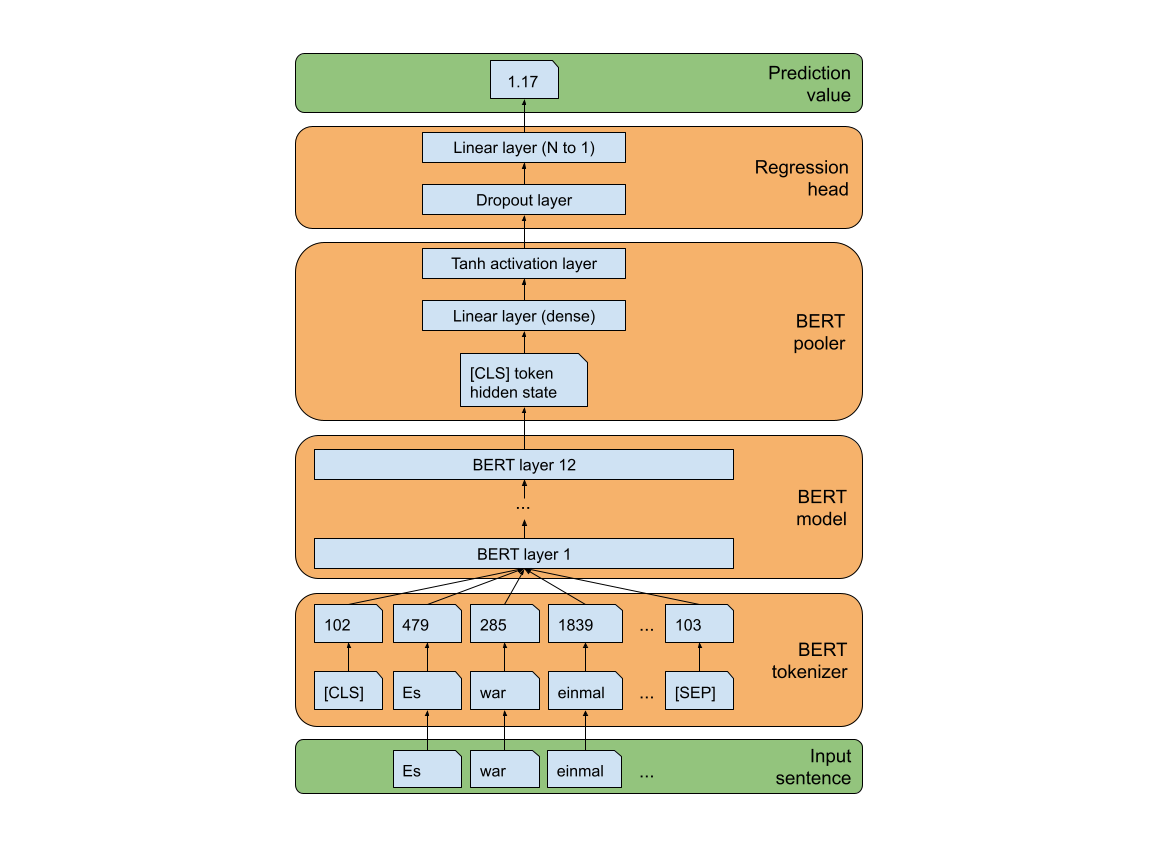
\includegraphics[width=\linewidth]{bert_regressor.png}
\caption{Diagram of the model architecture}
\label{fig:diag_model}
\end{figure}


\section{Tables}
\label{appendix:tables}

\begin{table}[h]
\center
  \begin{tabular}{l|cc}
    hyperparameter & value & \\
    \hline
    number of epochs & \(3\) & \\
    batch size & \(16\) & \\
    learning rate init & \(5\mathrm{e}{-5}\) & \\
    learning rate decay & linear & \\
    optimizer parameters & default &
  \end{tabular}
  \caption{Hyperparamters for training (fine-tuning)}
  \label{tab:train_hyperparams}
\end{table}

\end{appendices}


\end{document}
